\documentclass{jsarticle}
\usepackage[dvipdfmx]{graphicx}
\usepackage{amsmath,amssymb}

\newcommand{\argmax}{\mathop{\rm arg~max}\limits}
\newcommand{\argmin}{\mathop{\rm arg~min}\limits}

\begin{document}

\title{Matrix Profile I: All Pairs Similarity Joins for Time Series:\\
	A Unifying View that Includes Motifs, Discords and Shapelets}
\author{著者:hin-Chia Michael Yeh, Yan Zhu, Liudmila Ulanova, Nurjahan Begum, Yifei Ding,\\
	Hoang Anh Dau, Diego Furtado Silva, Abdullah Mueen, and Eamonn Keogh}
\date{}
\maketitle
会議名,年: IEEE 16th International Conference on Data Mining (ICDM), 2016
\section{概要}
\subsection{どんな論文?}
1本の時系列から部分時系列とその最近傍の部分時系列との距離・インデックスを格納するMatrix Profileを提案

\subsection{Matrix Profileとは}
長さ$n$の時系列$\boldsymbol{T}$から部分時系列の長さ$m$を決め,任意の部分時系列とその最近傍の部分時系列の距離とインデックスを格納する。\\
インデックス$i$で始まる長さ$m$の時系列を$t_{i,m}$と表すと,
\begin{displaymath}
\mathrm{MP}_i = \min_j{\mathrm{ED}(\mathrm{zscore}(\boldsymbol{T}_{i,m}),\mathrm{zscore}(\boldsymbol{T}_{j,m}))},
\end{displaymath}
\begin{displaymath}
\mathrm{MPIndex}_i = \argmin_j{\mathrm{ED}(\mathrm{zscore}(\boldsymbol{T}_{i,m}),\mathrm{zscore}(\boldsymbol{T}_{j,m}))}
\end{displaymath}
となる($\mathrm{zscore}(\boldsymbol{t})$は,$\boldsymbol{t}$を正規化することを指す).



\begin{itemize}
	\item Matrix Profileの例\\
	matrix profileの値が低いところ → 類似した部分時系列が存在する\\
\begin{figure}[h]
	\begin{center}
		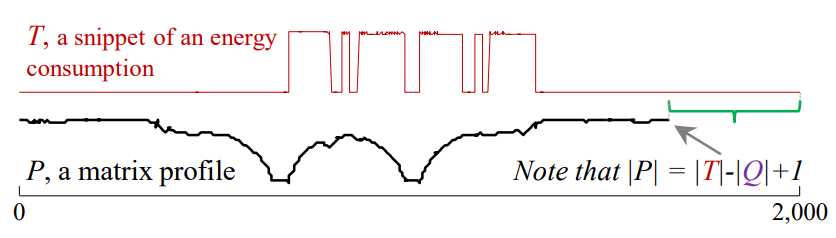
\includegraphics[scale = 0.50]{matrix_profile_fig3.png}
	\end{center}
	\caption{energy consumptionデータのmatrix profile(上:時系列データ,下:MatrixProfile)}
%	\label{fig:sleep_example}
\end{figure}


	反対にmatrix profileの値が高いところは他に類似した部分時系列がないので,異常検知などにも応用できる可能性がある
\begin{figure}[h]
	\begin{center}
		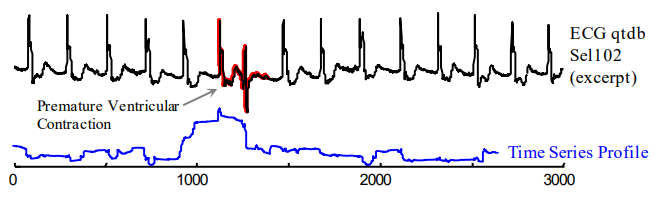
\includegraphics[scale = 0.6]{matrix_profile_fig13.png}
	\end{center}
	\caption{ECGデータのmatrix profile(上:時系列データ,下:MatrixProfile)}
%	\label{fig:sleep_example}
\end{figure}
\end{itemize}


\subsection{似ている手法}
\begin{itemize}
	\item k近傍法
\end{itemize}

\subsection{メリット}
\begin{itemize}
	\item 視覚的にモチーフになり得る箇所が分かる
	\item 愚直に計算すると$O(mn^2)$だが,高速化により$O(n^2)$に削減できる
\end{itemize}

\section{感想・メモ}
\begin{itemize}
	\item モチーフとなり得る箇所などが視覚的に理解できるという点で、時系列マイニングに非常に有効だと感じた
	\item 高速化をしても計算オーダーが$O(n^2)$なので,長すぎる時系列に適用するにはデータを削減するなどして対応する必要がある
	\item 高速化の部分がまだ理解していないので勉強中
\end{itemize}
\end{document}

\end{document}